\documentclass[11pt]{beamer}
\usetheme{Marburg}
%\usecolortheme{beaver}
\usepackage[utf8]{inputenc}
\usepackage[german]{babel}
\usepackage[T1]{fontenc}
\usepackage{amsmath}
\usepackage{amsfonts}
\usepackage{kpfonts}
\usepackage{float}
\usepackage{amssymb}
\usepackage{graphicx}
\setbeamertemplate{footline}[page number]
\author{Ronja van Luijt\\ Nick Jannis Schmeißer}
\title{Projekt Torsionspendel}
\setbeamercovered{transparent} 
\graphicspath{ {images/} }
\setbeamertemplate{navigation symbols}{} 
%\logo{} 
\institute[BUW]{Bergische Universität Wuppertal} 
\date{08.07.2019} 
%\subject{} 
\begin{document}

\begin{frame}
\titlepage
\end{frame}

\begin{frame}
\frametitle{Inhaltsverzeichnis}
\tableofcontents
\end{frame}

\section{Idee und Vorbereitung}
\subsection{Zielsetzung}
\begin{frame}
\frametitle{Idee und Vorbereitung}
\begin{itemize}
\item Erinnerung Praktikum AP1a M3:\pause
\item Torsionspendel:
\begin{itemize}
\item Querstange an Draht befestigt
\item zwei zylinderförmige Massen an der Stange\\mit gleichem Abstand zum Draht
\item Bei Auslenkung führt die Konstruktion eine Schwingung durch
\end{itemize}\pause
\item Ziel:
\begin{itemize}
\item Trägheitsmoment der Konstruktion berechnen lassen
\item Richtmoment und Kreisfrequenz ausgeben lassen
\item Schwingung des Pendels simulieren
\item Auslenkungsgraph erstellen
\item Fehlerrechnung
\end{itemize}
\end{itemize}
\end{frame}

\begin{frame}
\frametitle{Bild}
\begin{figure} [H]
\centering
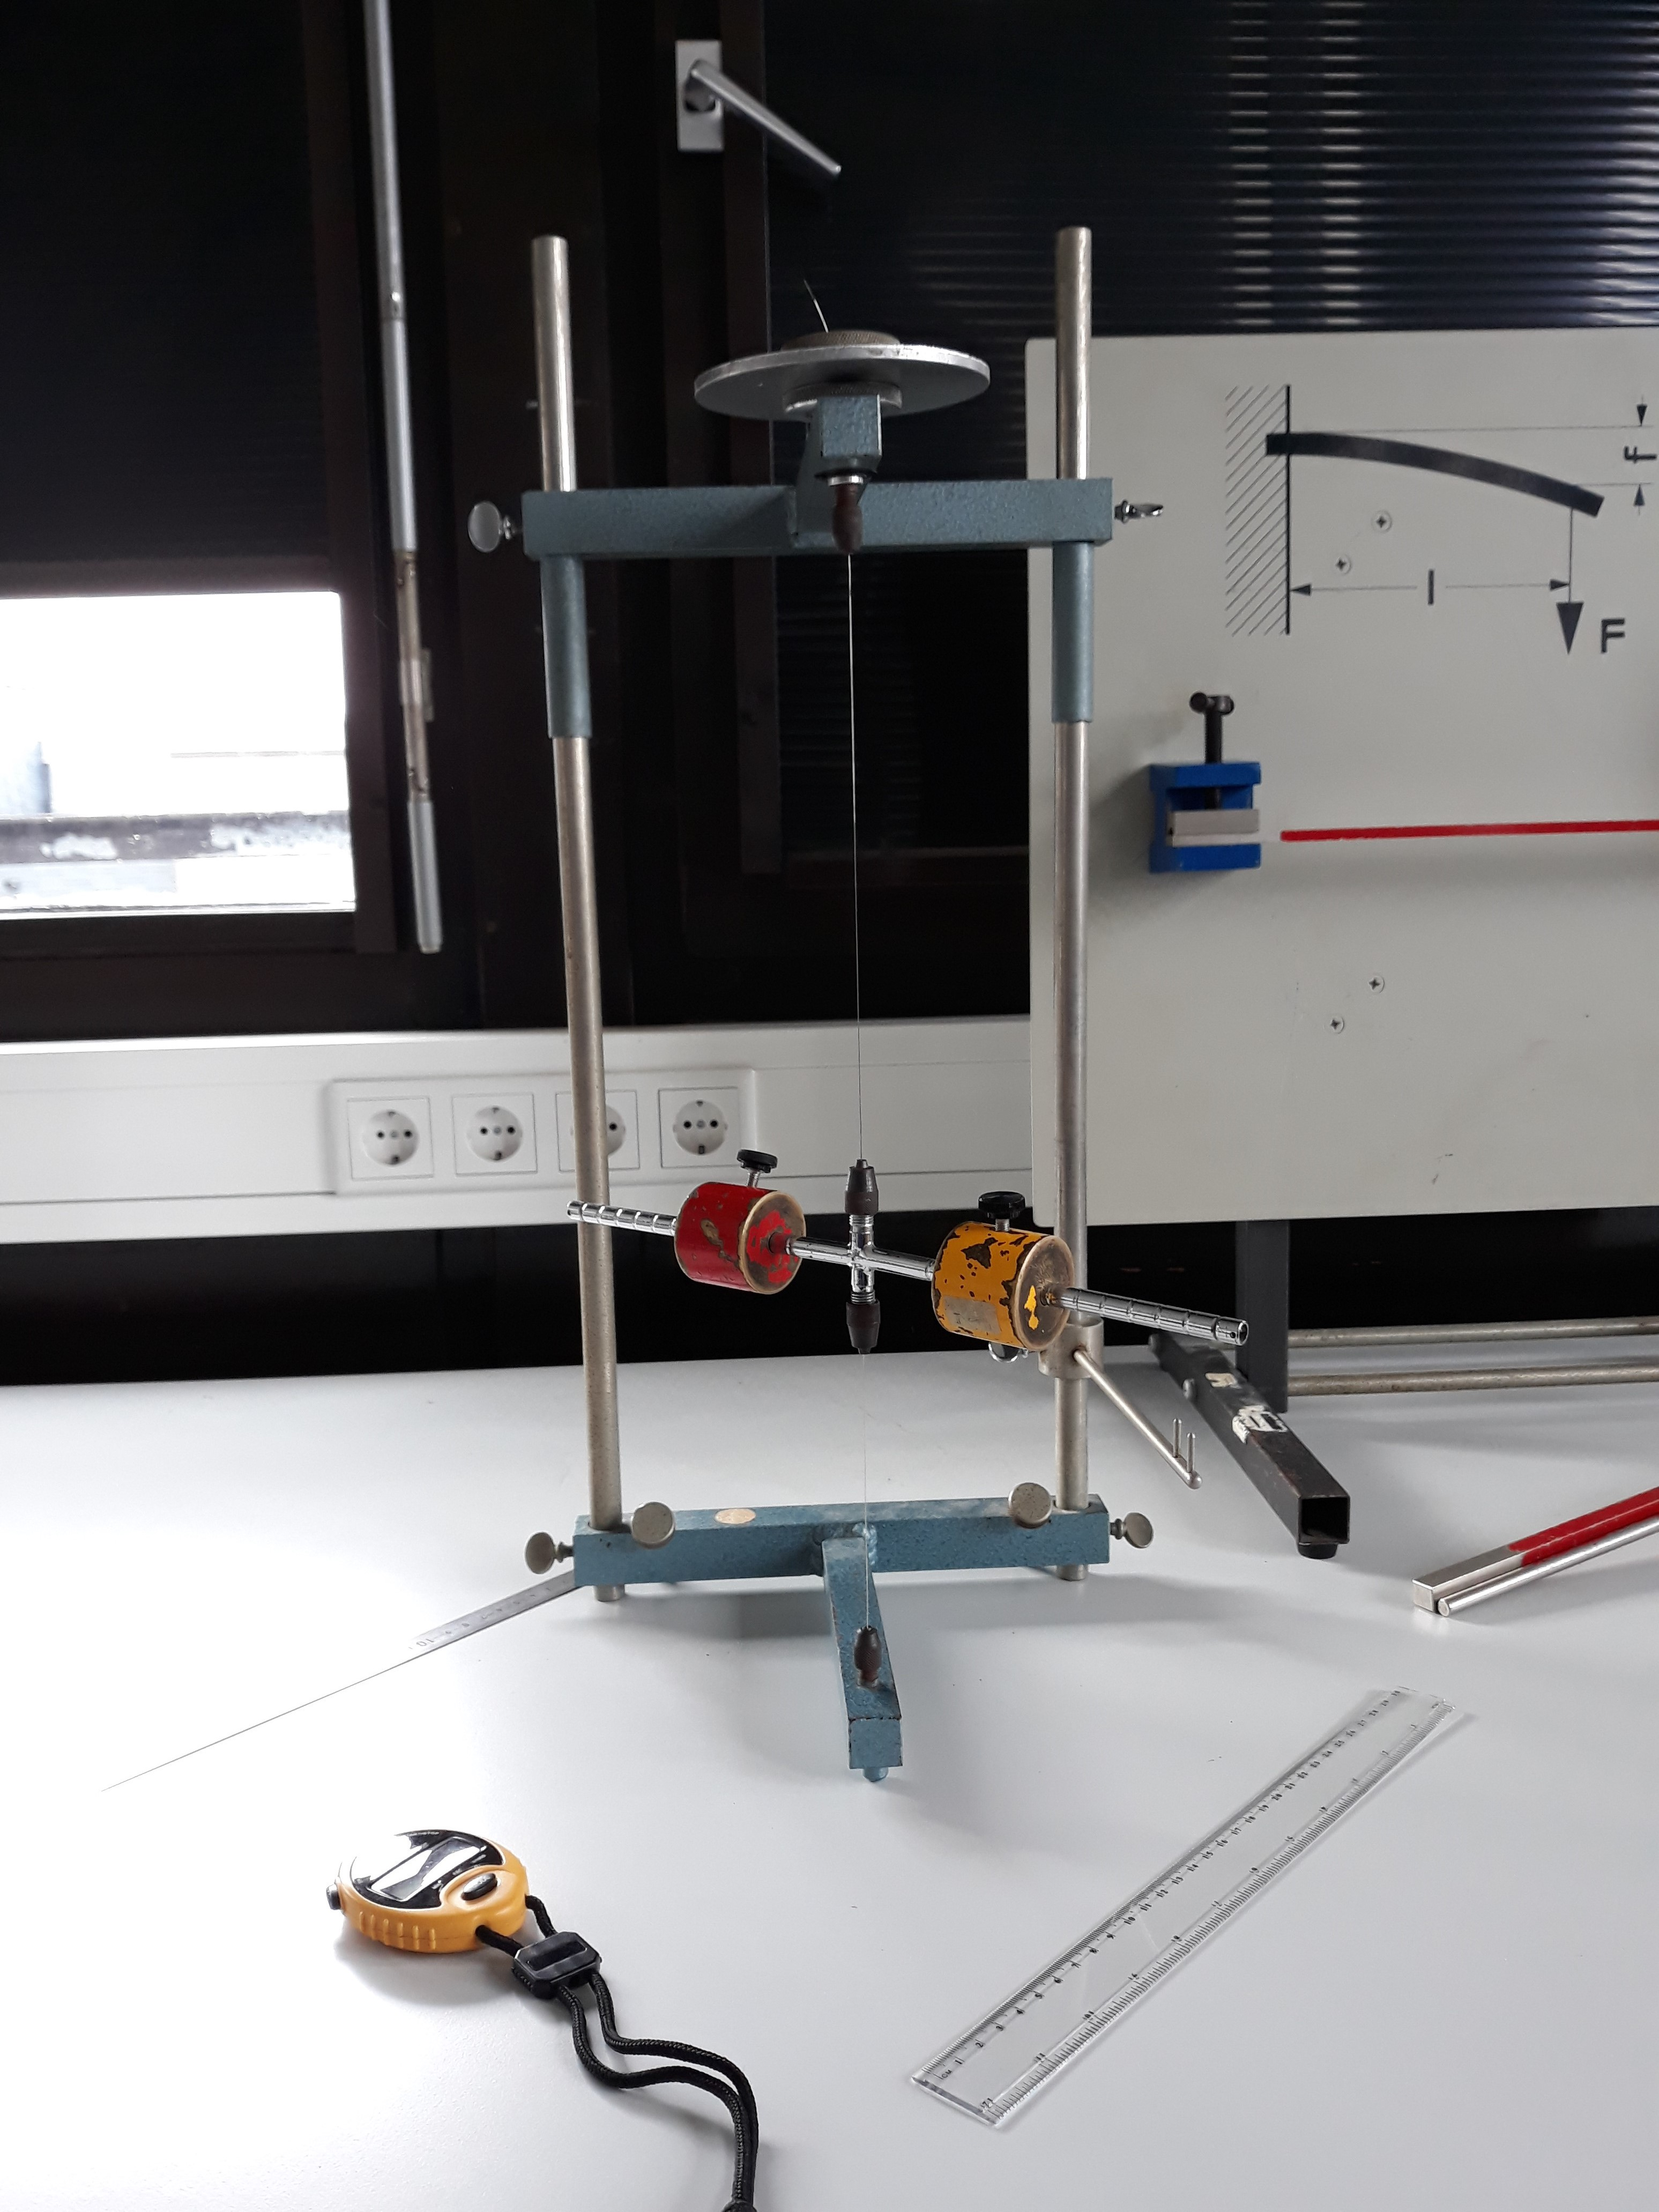
\includegraphics[width=0.75\textwidth]{Teil_2.jpg}
\caption{Dieses Bild zeigt ein Torsionspendel aus dem AP1a.}
\end{figure}
\end{frame}

\subsection{Planung}
\begin{frame}
\frametitle{Planung}
\begin{itemize}
\item Planung der Klassen:
\begin{itemize}
\item Pendel
\item Masse (für Hohlzylinder)
\item Draht
\item mainfile zur Kommunikation mit User
\end{itemize}\pause
\item Erstellen eines Repositories auf Github:
\item \url{https://github.com/NickJannis/Projekt_Torsionspendel}
\end{itemize}
\end{frame}

\section{Physikalischer Hintergrund}
\begin{frame}
\frametitle{Physikalischer Hintergrund}
\begin{itemize}
\item Lösung der Schwingungsgleichung:\\
\begin{equation}
\varphi(t)=A_m\cdot\sin{(\omega_0\cdot t+\frac{\pi}{2})}
\end{equation}
\item Lösen der Gleichung $\theta\ddot \varphi +D \varphi = 0$ liefert:
\item \begin{equation}
\omega = \sqrt{\frac{D}{\theta}}
\end{equation}
\item \begin{equation}
\theta = \theta_S +2\cdot \left(\theta_x + md^2\right)
\end{equation}
\item \begin{equation}
\theta_x = \frac{M}{4}\cdot \left(R_a^2+R_i^2+\frac{l^2}{3} \right)
\end{equation}
\item \begin{equation}
D=\pi G \frac{R^4}{2L}
\end{equation}
\end{itemize}
\end{frame}

\section{Klassenstruktur}
\begin{frame}
\frametitle{Klassenstruktur}
\begin{itemize}
\item Klasse Masse:\\Simuliert Hohlzylinder mit eigenem Trägheitsmoment
\item Klasse Draht:\\Simuliert Torsionsdraht mit Torsionsmodul(Schubmodul)
\item Klasse Pendel:\\Verbindet Masseelemente und Draht zum Pendel mit eigenem Trägheitsmoment und kann Auslenkung berechnen
\item Größen mit Fehler werden mit Datentyp $array<double, 2>$ gespeichert
\end{itemize}
\end{frame}

\subsection{Klassen}
\begin{frame}
\frametitle{Klasse Pendel}
\begin{figure} [H]
\centering
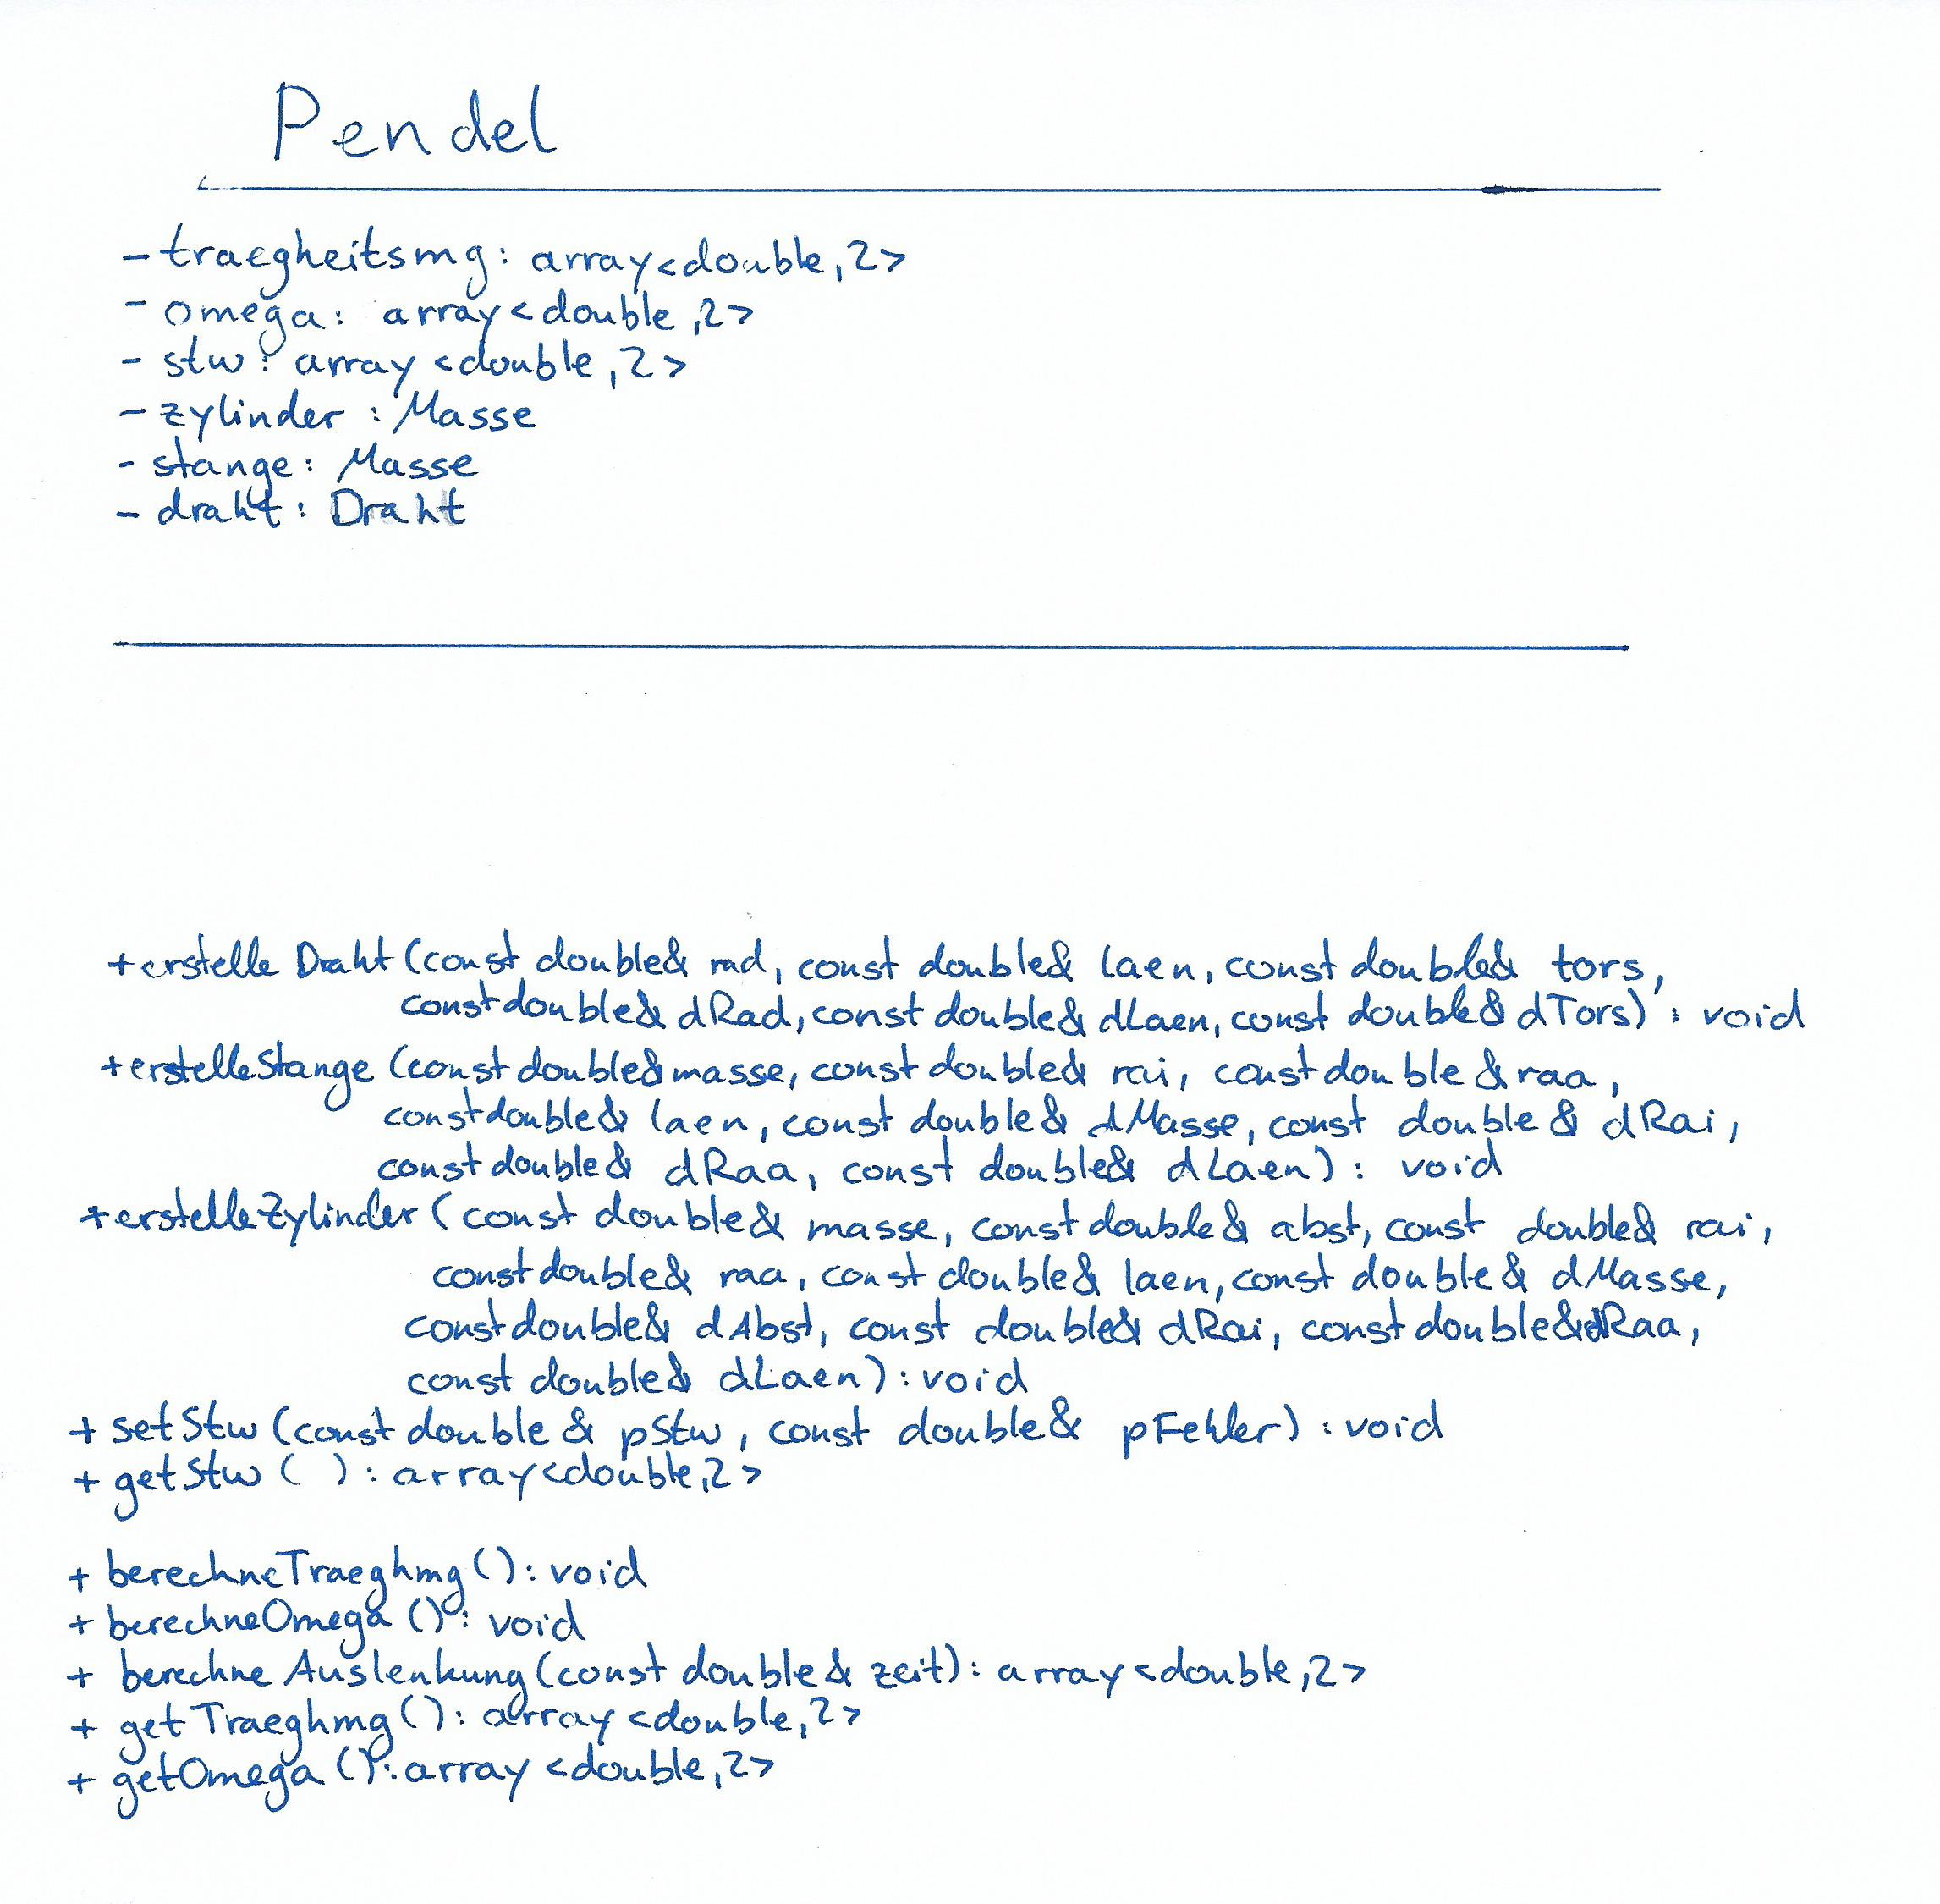
\includegraphics[width=0.9\textwidth]{info_1.jpg}
\caption{Klassenkarte der Klasse Pendel}
\end{figure}
\end{frame}

\begin{frame}
\frametitle{Das Main-File}
\begin{figure} [H]
\centering
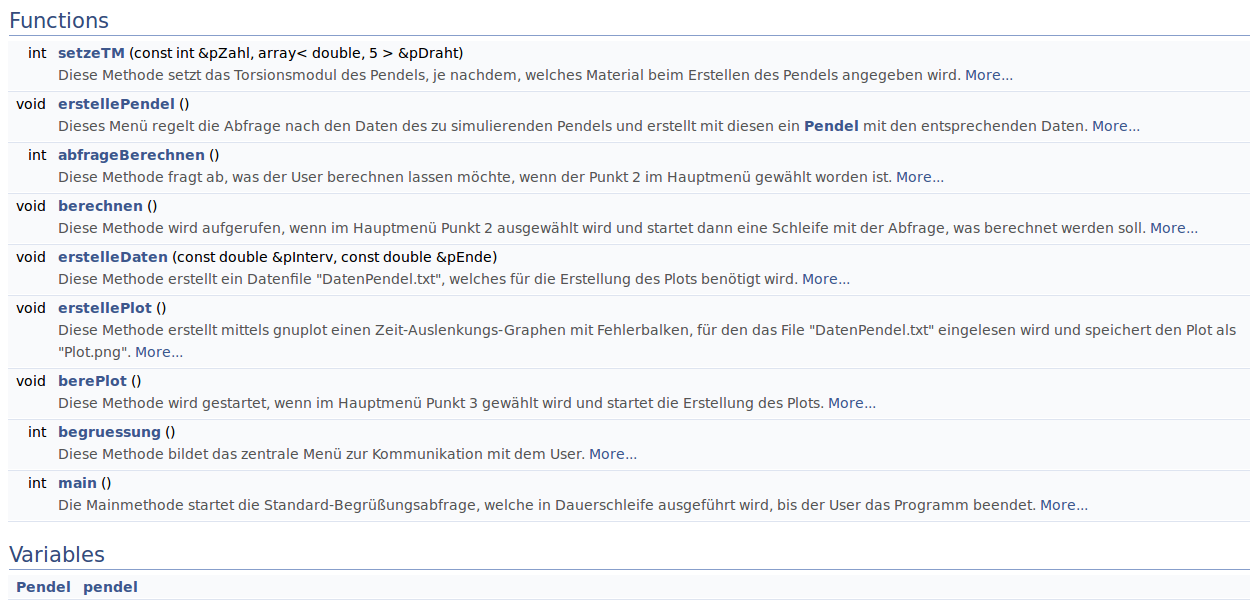
\includegraphics[width=0.9\textwidth]{main.jpg}
\caption{Dieses Bild zeigt einen Überblick aus dem Main-File.}
\end{figure}
\begin{itemize}
\item Dieses File organisiert Kommunikation zwischen User und Programm
\end{itemize}
\end{frame}

\begin{frame}
\frametitle{Das Hauptmenü}
\begin{figure} [H]
\centering
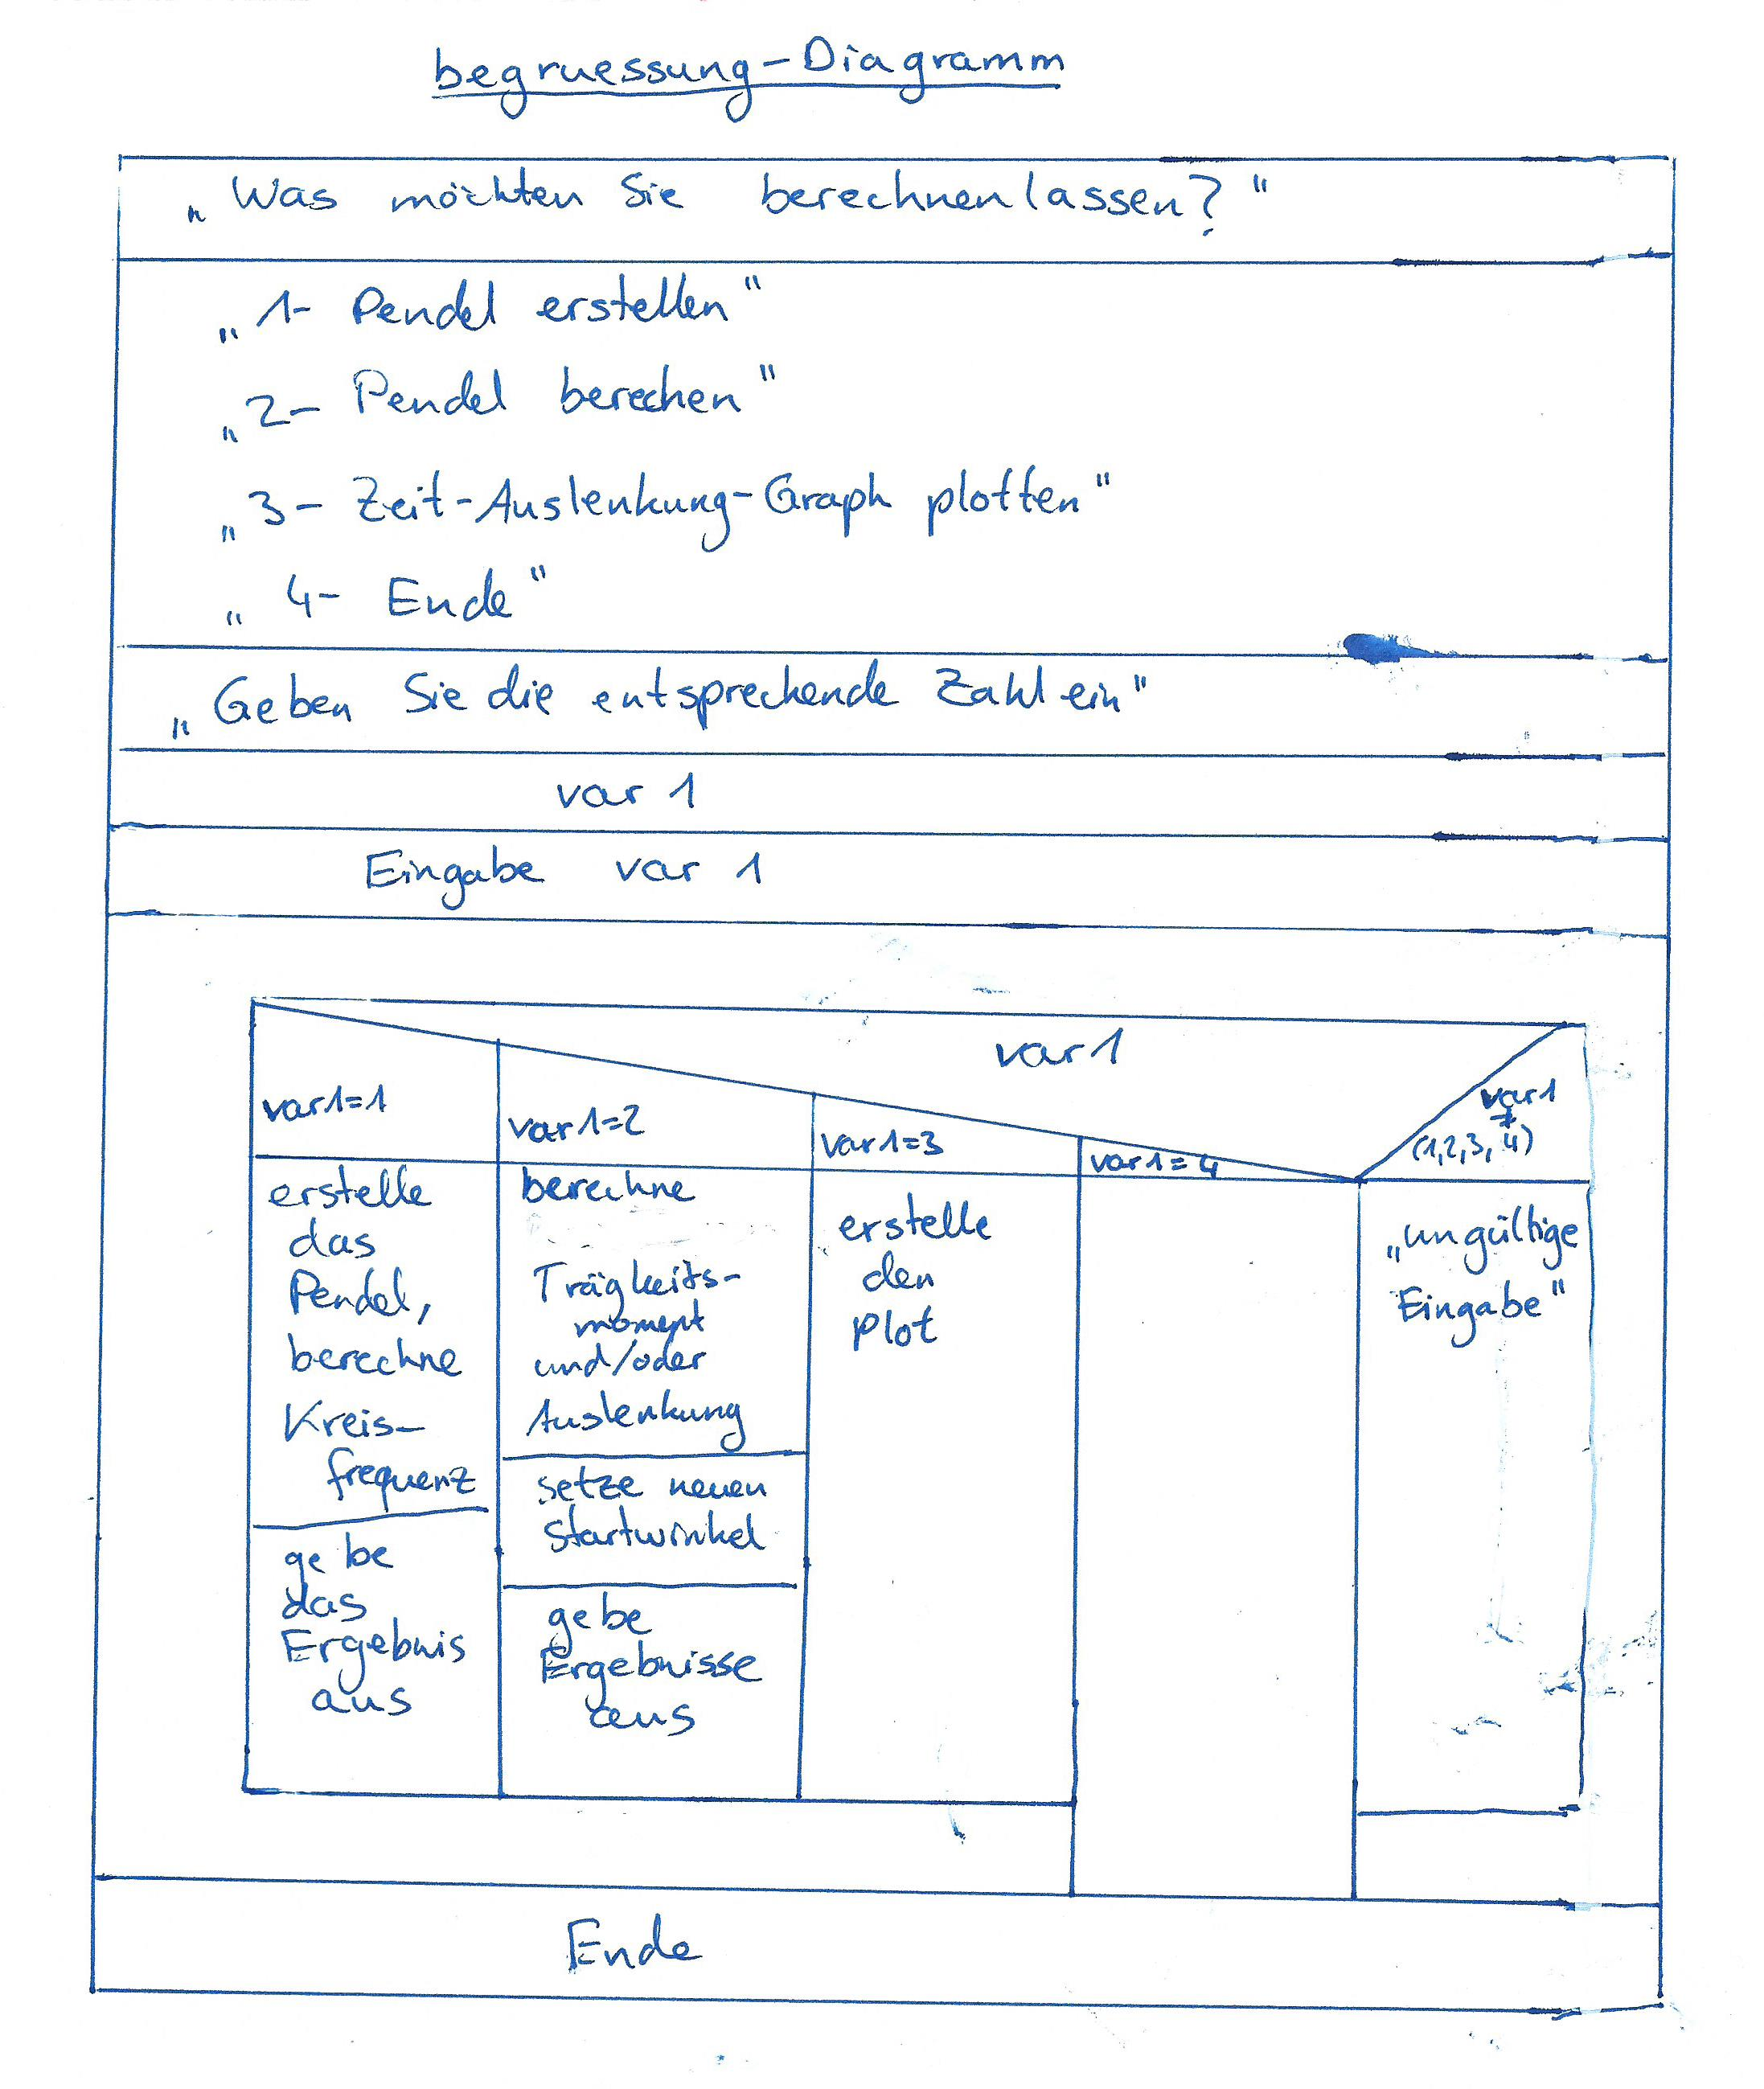
\includegraphics[width=0.75\textwidth]{info_2.jpg}
\caption{Begrüßungsmethode aus dem Mainfile, die das Hauptmenü bildet.}
\end{figure}
\end{frame}

\begin{frame}
\frametitle{Methode erstelleDaten}
\begin{figure} [H]
\centering
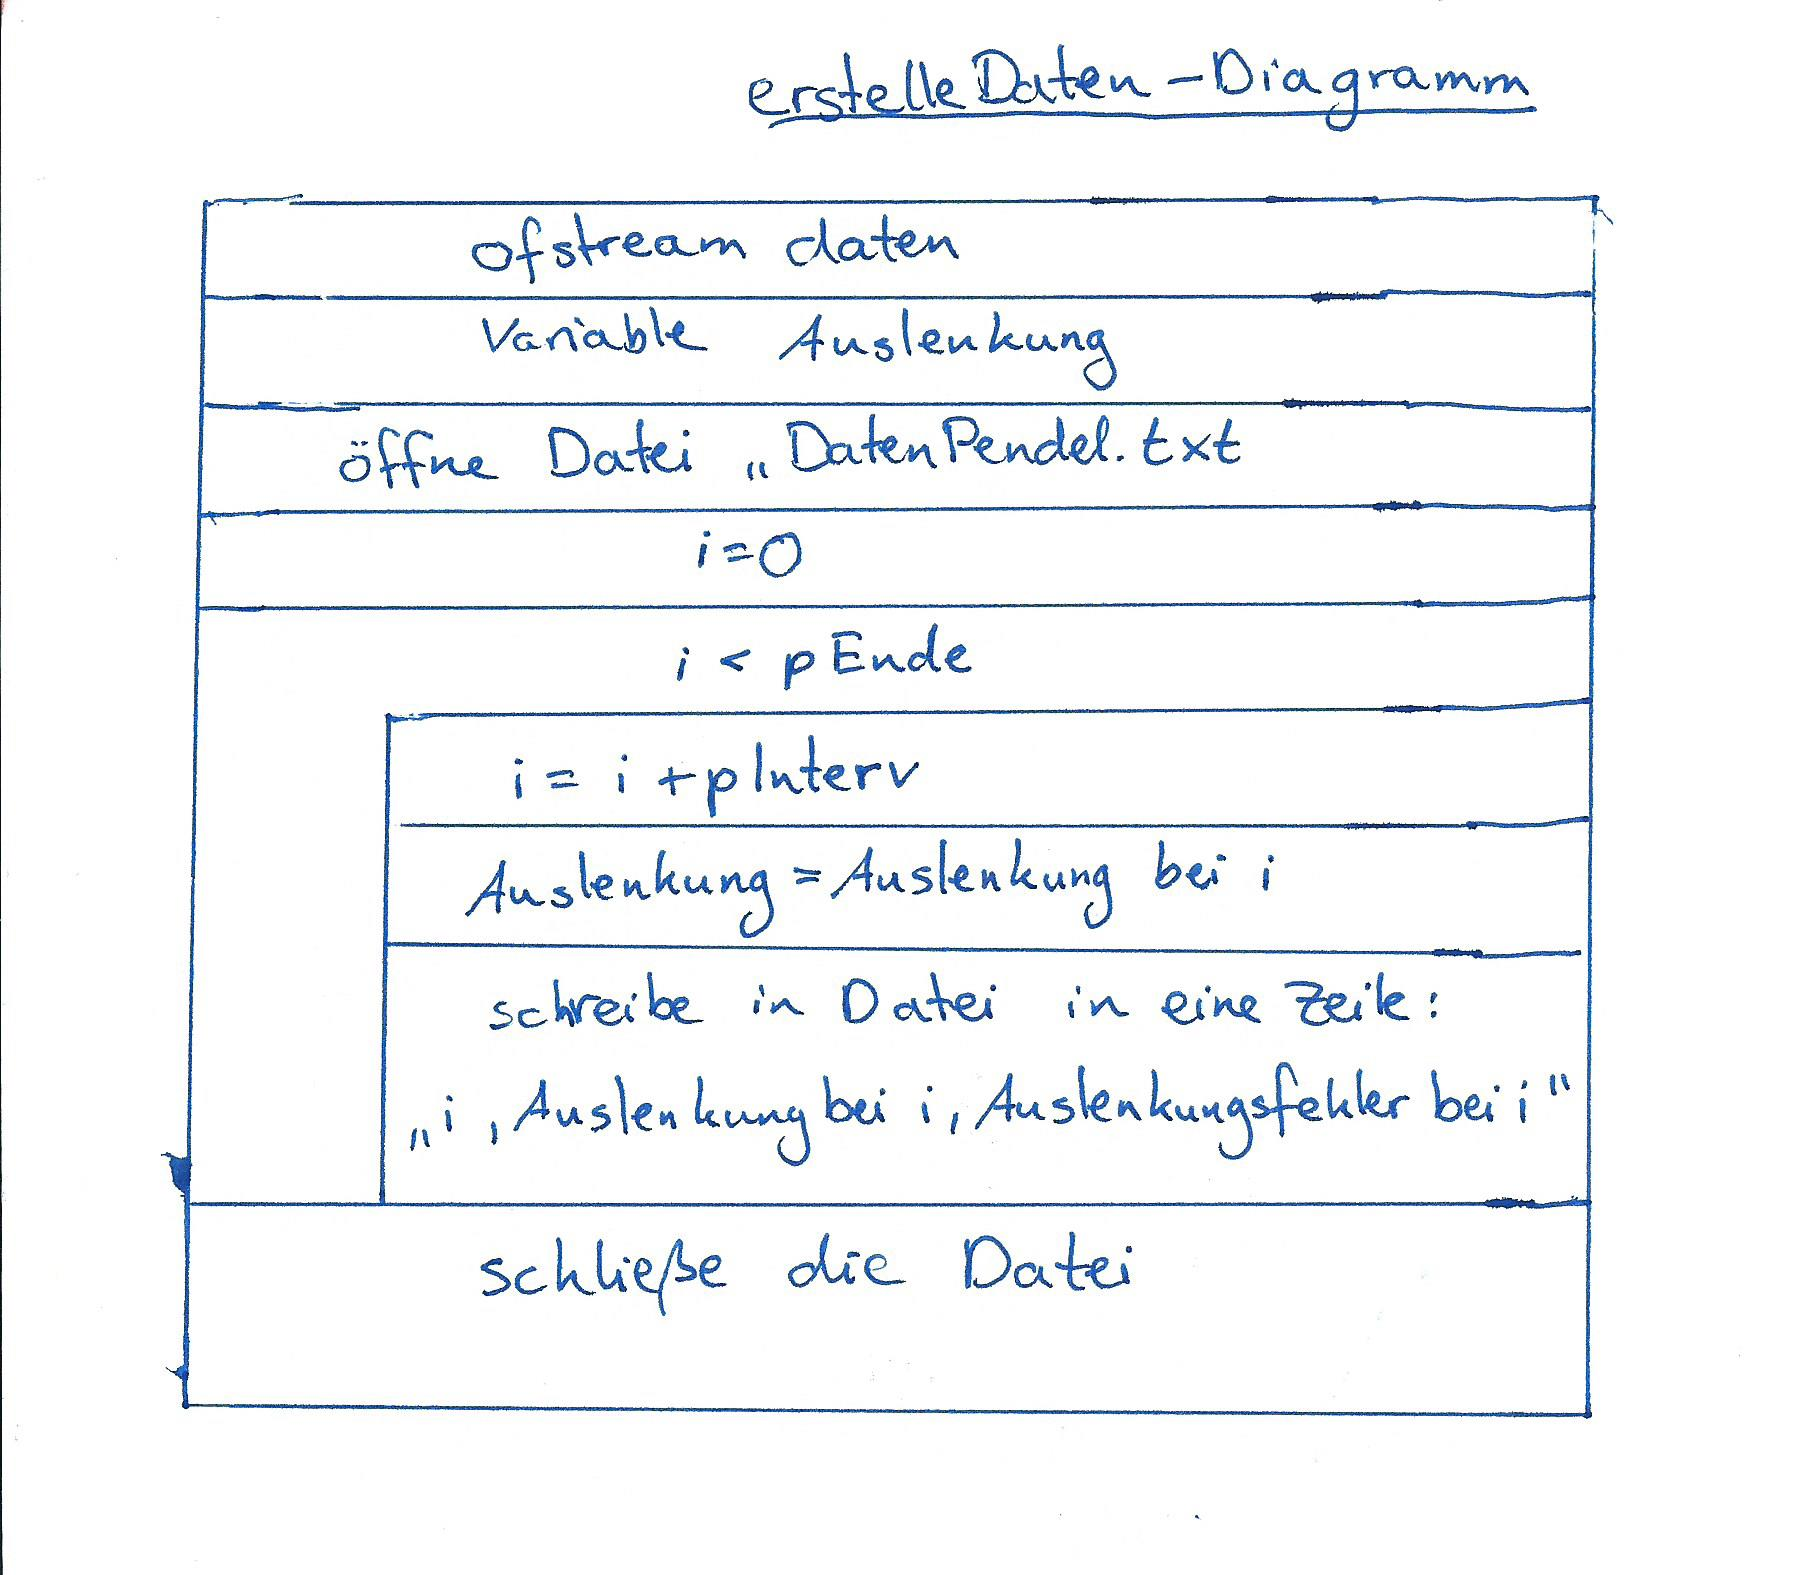
\includegraphics[width=0.8\textwidth]{info_3.jpg}
\caption{Methode zum Erstellen der Daten-Files}
\end{figure}
\end{frame}

\begin{frame}
\frametitle{Plot erstellen mit GnuPlot}
\begin{itemize}
\item Gnuplot per \url{gnuplot_i.hpp} in c++ einbinden
\item Quelle Befehle: \url{www.gnuplot.info}
\item Daten aus dem Datenfile einlesen und plotten mit Fehlerbalken
\end{itemize}
\begin{figure} [H]
\centering
\includegraphics[width=0.9\textwidth]{Gnuplot.jpg}
\caption{Einbindung von Gnuplot in c++}
\end{figure}
\end{frame}

\begin{frame}
\frametitle{Klasse Masse}
\begin{itemize}
\item Simuliert die Eigenschaften eines Hohlzylinders
\item Attribute:
\begin{figure} [H]
\centering
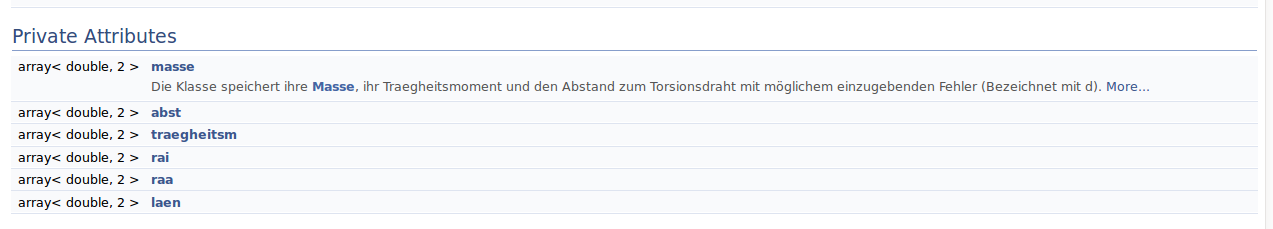
\includegraphics[width=0.9\textwidth]{Masse2.jpg}
\caption{Dieses Bild zeigt die Attribute der Klasse Masse.}
\end{figure}
\end{itemize}
\end{frame}

\begin{frame}
\frametitle{Klasse Masse}
\begin{figure} [H]
\centering
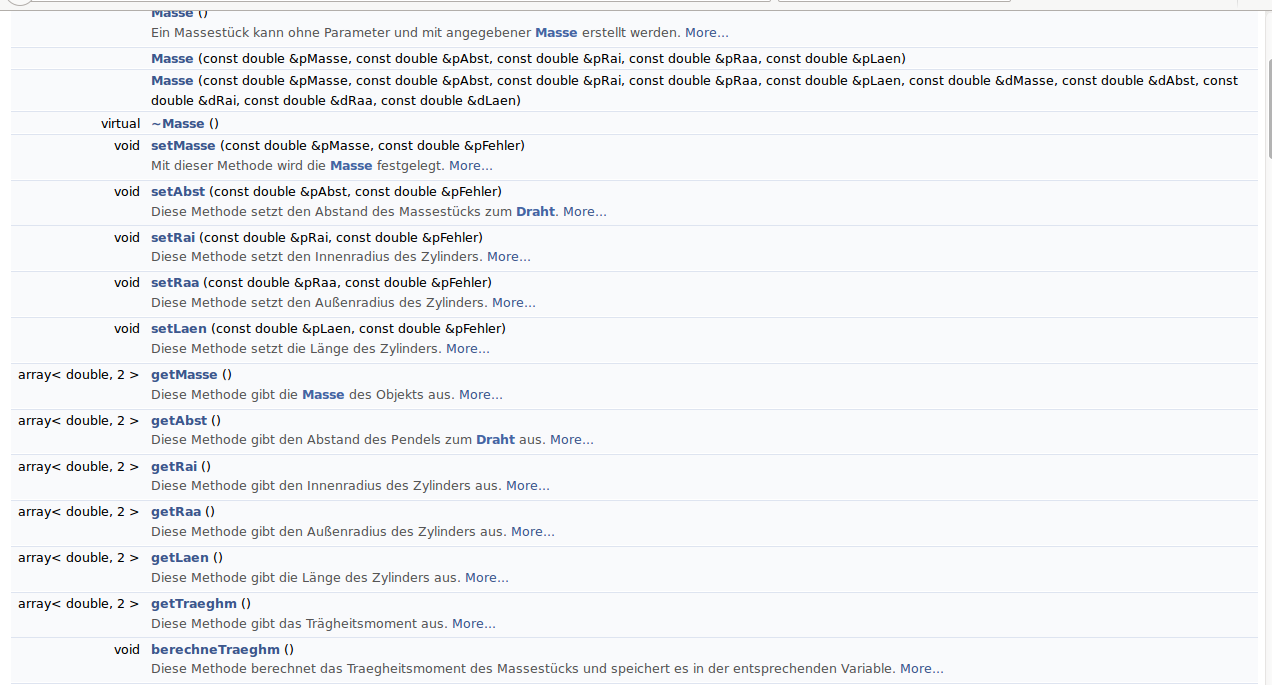
\includegraphics[width=0.9\textwidth]{Masse.jpg}
\caption{Dieses Bild zeigt die Methoden der Klasse Masse.}
\end{figure}
\end{frame}

\begin{frame}
\frametitle{Klasse Draht}
\begin{itemize}
\item Simuliert Draht:
\begin{itemize}
\item Torsionsmodul
\item Richtmoment
\end{itemize}
\end{itemize}
\begin{figure} [H]
\centering
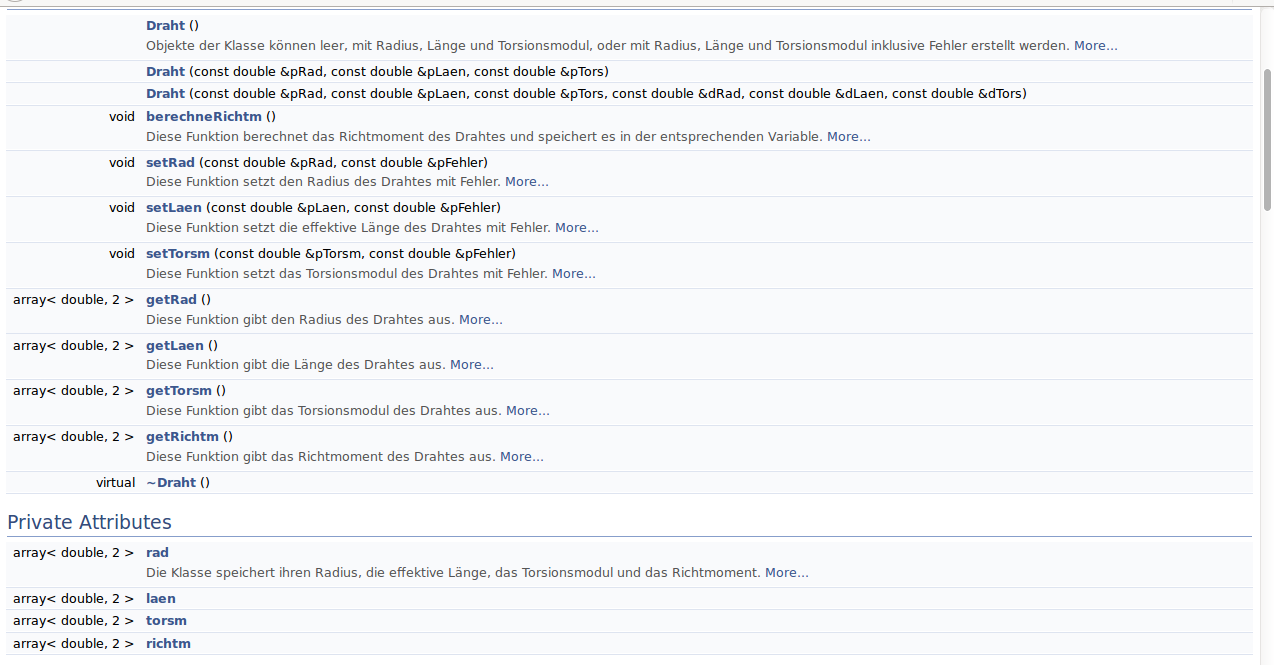
\includegraphics[width=0.9\textwidth]{Draht.jpg}
\caption{Dieses Bild zeigt die Klasse Draht.}
\end{figure}
\end{frame}

\section{Kompilieren und Ausführen}
\begin{frame}
\frametitle{Kompilieren und Ausführen}
\begin{itemize}
\item Kompilieren mit c++11
\item Alternativ existiert ein Makefile:
\item Kompilieren mit make
\item Ausführen mit ./Pendel.out
\end{itemize}
\end{frame}

\subsection{Bedienungsbeispiel}
\begin{frame}
\frametitle{Bedienungsbeispiel: kompilieren und starten}
\begin{figure} [H]
\centering
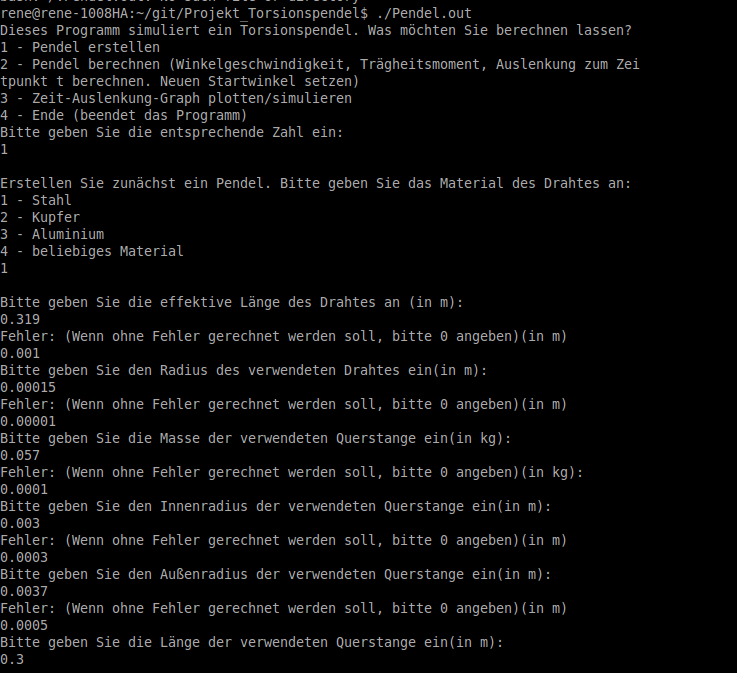
\includegraphics[width=0.8\textwidth]{Teil_a.jpg}
\caption{Dieses Bild zeigt, wie das Programm zu starten ist.}
\end{figure}
\end{frame}

\begin{frame}
\frametitle{Erstellen eines Pendels}
\begin{figure} [H]
\centering
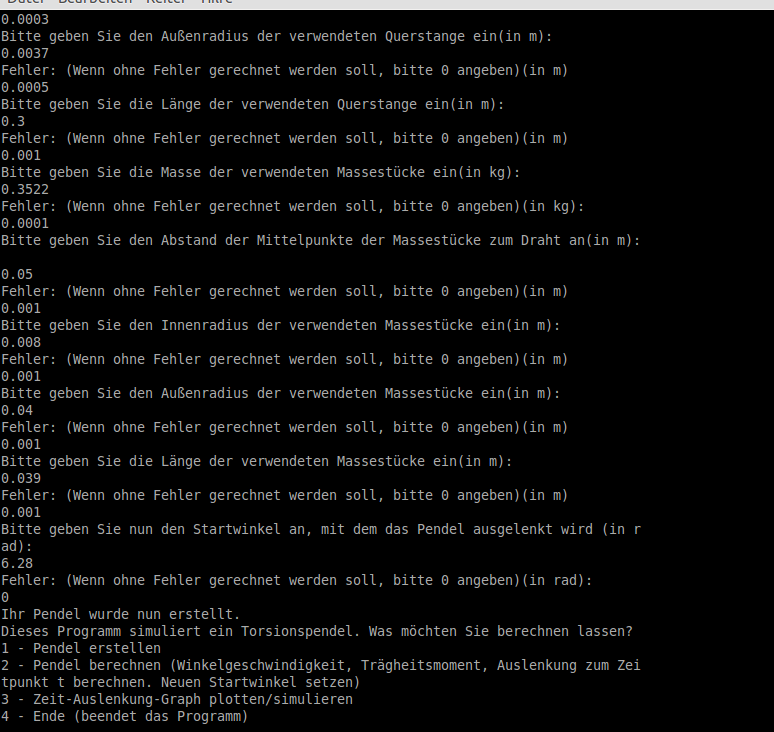
\includegraphics[width=0.8\textwidth]{Teil_b.jpg}
\caption{Die Abfragen werden nacheinander durchgeführt.}
\end{figure}
\end{frame}

\begin{frame}
\frametitle{Berechnungen}
\begin{figure} [H]
\centering
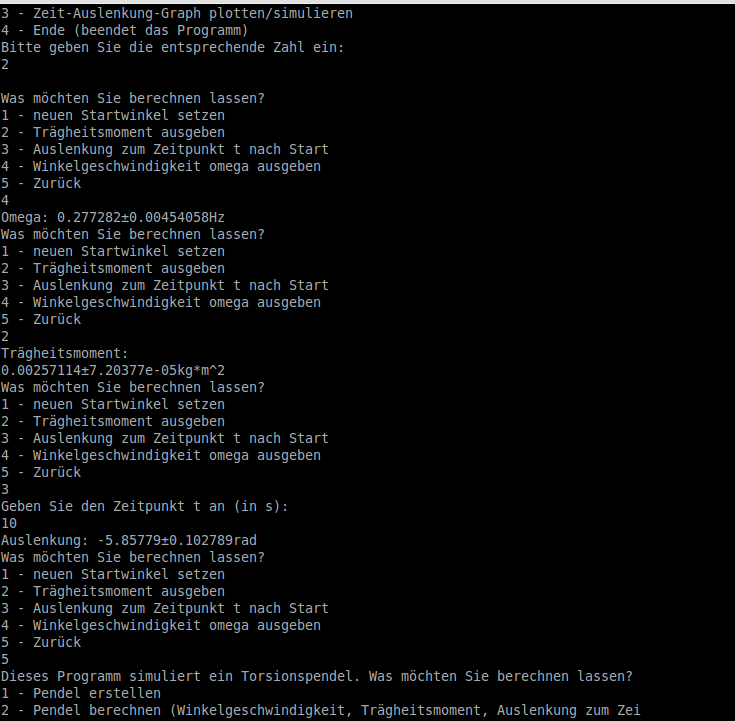
\includegraphics[width=0.7\textwidth]{Teil_c.jpg}
\caption{Es können das Trägheitsmoment, die Kreisfrequenz und die Auslenkung zu einem bestimmten Zeitpunkt ausgegeben werden.}
\end{figure}
\end{frame}

\begin{frame}
\frametitle{Plot erstellen}
\begin{itemize}
\item Intervalle zwischen den Datenpunkten und Zeitraum können angegeben werden
\end{itemize}
\begin{figure} [H]
\centering
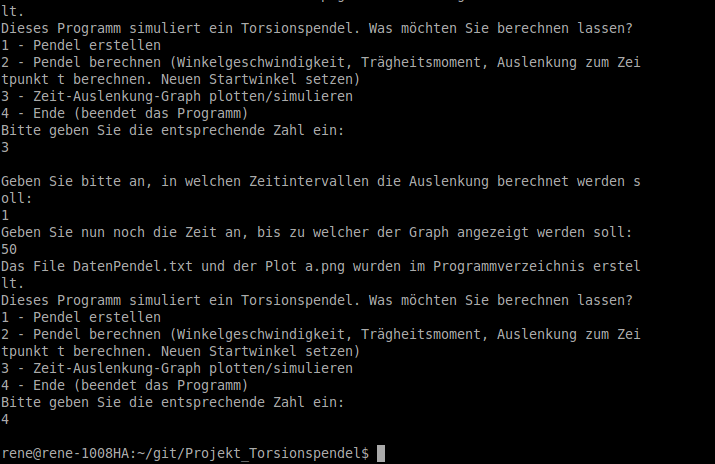
\includegraphics[width=0.9\textwidth]{Teil_z.jpg}
\caption{Bei Eingabe von 4 im Hauptmenü wird das Programm beendet.}
\end{figure}
\end{frame}

\begin{frame}
\frametitle{Daten-File}
\begin{itemize}
\item Gespeichert werden Zeit, Auslenkung und Fehler der Auslenkung in 3 Spalten
\end{itemize}
\begin{figure} [H]
\centering
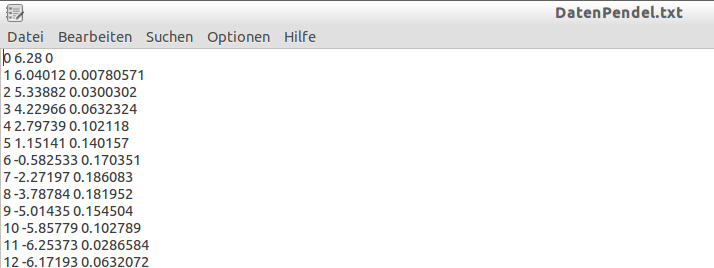
\includegraphics[width=0.9\textwidth]{Daten.jpg}
\caption{Ein Ausschnitt aus den Daten}
\end{figure}
\end{frame}

\begin{frame}
\frametitle{Plot}
\begin{figure} [H]
\centering
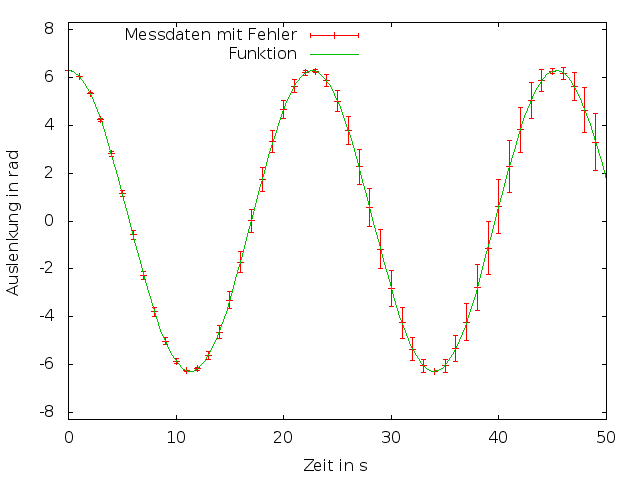
\includegraphics[width=0.9\textwidth]{Plot.png}
\caption{Der beim Beispiel erstellte Plot mit Intervallen 1s und Zeitraum 50s.}
\end{figure}
\end{frame}

\end{document}